\documentclass[11pt]{article}
\usepackage[a4paper, total={6.5in, 9.5in}]{geometry}
\usepackage[document]{ragged2e}
\usepackage[bookmarksopen=true,hidelinks]{hyperref}
\usepackage{bookmark}
\usepackage{lipsum}
\usepackage{graphicx}
\usepackage{float}
\usepackage[numbib]{tocbibind}
\usepackage{multirow}
\usepackage{array}
\usepackage{setspace}
\usepackage{cellspace}
\usepackage{etoolbox}
\usepackage{longtable}
\usepackage[table, svgnames]{xcolor}
\usepackage{titlesec}
\usepackage{amsmath}
\usepackage{pdfpages}
\setcounter{secnumdepth}{4}
\usepackage{fancyhdr}
\fancypagestyle{logo}{
    \fancyhf{} % clears header/footer
    \renewcommand\bottomfraction{0.9}
    \renewcommand\textfraction{0.1}
    \fancyhead[C]{
\includegraphics[ width=\linewidth, keepaspectratio]{./images/header_white.png}}
    \fancyfoot[LE,RO]{\thepage}
}
\pagestyle{logo}


%\usepackage[noadjust]{cite}
\usepackage[sorting=none, backend=biber]{biblatex}
\addbibresource{bibi_uid.bib} 


\begin{document}
\

\setcounter{section}{9}
\section{Appendix B: User Interface and Appearance}
\bigskip


\subsection{Introduction}
\medskip
The User Interface Design Appendix provides a detailed description and analysis of the Akriveia Beacon System in terms of the design, communication, and operations with the intended users. The Akriveia Beacon system is an advanced indoor location rescue system designed to aid first responders during an emergency search and rescue situation by providing accurate location of trapped victims within commercial buildings. The primary users to interact with the Akrievia Beacon system will be first responders such as fire fighters or emergency management personnel. The secondary users to interact with the system would be administrators or IT technicians that would utilize or perform maintenance and upkeep of the system. Lastly, the tertiary users would be the employees of the company using the Akriveia Beacon system. The employee will only interact with the system by turning the ID tags on during an emergency. Since the system is intended to operate under extremely stressful environments and situations, the user interface must be as clear and intuitive to use as possible to ensure that first responders can operate at peak efficiency along side the Akriveia Beacon system.
\bigskip

\subsubsection{Purpose}
\medskip
The focus of this user interface design appendix is to act as a reference for engineers at TRIWAVE SYSTEMS throughout development. In order to create an interface that is both clear and intuitive for the intended user, the hardware and software interfaces must follow strict design standards and requirements. Such standards and requirements will ensure that during the intended operating scenario, the system would not cause users unexpected error due to implications of insufficient operating knowledge or unforeseeable circumstances. These design requirements will be presented in conjunction with the three specific development phases: the proof-of-concept phase, prototype phase, and the Final product phase.
\bigskip

\subsubsection{Scope}
\medskip
This document includes detailed overview of user and technical analysis, engineering safety and standards, and usability testing in order to provide sufficient understanding of the user interface for the Akriveia Beacon system. As a system to be operating under disaster or emergency situations, the Akriveia Beacon must require some form of basic user knowledge in order for different parties of the user base to operate the system sufficient. Outline of the required user knowledge allowing basic usage of the Akriveia Beacon system will be presented. As well as the following seven fundamental technical analysis principles will be considered when making design choices for the user interface: discoverability, feedback, conceptual models, affordances, signifiers, mappings, and constraints; as outlined from Don Norman's The Design of Everyday Things. Finally, the appendix will include analytical and empirical system test plans with different scenarios that is aimed at testing how the Akriveia Beacon system would operate under each specified condition during each stage of the development cycle. The test cases covered will provide additional quality assurance of the final product to ensure that the Akriveia Beacon system is both accurate and reliable for its intended purpose.







\pagebreak


\subsection{User Analysis}
\medskip
The Akriveia Beacon system has two main targeted users: emergency first responders, and the IT or systems administrators. Emergency first responders are considered to be the primary users as the system is designed to operate under emergency situations involving these personnels. For Emergency first responders the system will provide a very high level layer of interaction, where only the most necessary interaction are provided allowing intuitive access and decreasing the probability for mistakes. The system/IT administrators, the secondary users, are the personnels that will provide maintenance and upkeep of the system. Tasks such as managing user accounts for ID tags, performing system wide maintenance for the beacons and data processing units, and any potential upgrade, repair, and replacement procedures will be performed by these users. 
\bigskip


\subsubsection{User - Emergency First Responders}
\medskip
The primary users of the Akriveia system are the emergency first responders who are the first to arrive and provide assistance at the scene of an emergency, such as an accident or disaster. First responders typically include paramedics, emergency medical technicians, police officers, fire-fighters, rescuers, and other trained members of organisations. In the intended situation where a search and rescue operation will be performed, the targeted primary user to be interacting with the system will be considered to be the person who is the top executive rank or commanding officer in a fire department, or the Fire Chief. The fire chief will cover the standard operating guidelines (SOGs) include basic communications with fire-fighter units deployed into buildings. 
\medskip
For the primary user, brief background knowledge on the operation of basic electronic equipment such as laptops and tablets are essential. Since the main user interaction between the primary user and the Akriveia Beacon system is through a graphical user interface hosted on these basic electronic equipment, the user is required to have some form of familiarity with the equipment. Once the system is incorporated more into current infrastructure, training could also be provided to the primary users. Furthermore, basic comprehension of blueprint reading and ability to recognition and understanding of simple legends, icons, and other associated information on the user interface is required. In addition, the primary users should have the grammatical prowess to understand the English language, as well as familiarity with handling electronic devices such as laptops and tablets. Having fulfilled these mentioned user requirements, the primary users can optimally benefit from the Akriveia Beacon system.
\bigskip


\subsubsection{User - IT/systems administrators}
\medskip
The secondary users of the Akriveia system are the system administrators or IT technician that will be 
performing registration, maintain and upkeep of the system. For secondary users, formal technical background is required to perform system maintenance and upgrades. The secondary users will perform installation and configure appropriate software and functions according to specifications. As well as to ensure the security and privacy of the networks and computing systems. Their primary tasks include managing ID tag accounts associated with employees, perform inspection of equipment such as beacons, ID tags, and data processing unit. As well as to ensure functionality of the system by enabling and operating the system during disaster drills. Operational training for secondary users will be provided if necessary.








\pagebreak


\subsection{Technical Analysis}
\bigskip
This section will analyze the consideration for Seven Elements of UI Interface as outlined by Don Norman for the Akriveia Beacon system; which includes the following design factors, discoverability, feedback, conceptual models, affordances, signifiers, mappings, and constraints \cite{R10-3-1}. By incorporating these design element in to the system, the usability and quality of the final product can be substantially improved. 
\medskip

\subsubsection{Discoverability}
\medskip
Discoverability: Is it possible to even figure out what actions are possible and where and how to perform them?  In the context of product and interface design, discoverability is the degree of ease with which the user can find all the elements and features of a new system when they first encounter it \cite{R10-3-2}. The Akrivia beacon system is designed to operate under emergency situations and disasters, which means that it is paramount that the UI creates discoverability for its users. The overall interaction should be simple enough for each level of users to comprehend and understand without the need for much interpretation. 

\bigskip
Primary user - First Responders’ main point of interaction with the Akriveia Beacon system is through the GUI. The GUI will be simple with intuitive design allowing for quick understanding of the system and any relating concepts. For prototype UI design, the interface will be quick to access  and contains a scaled blueprint of the structure with colored indicators will conveying the location of victims on the map view (similar to figure \ref{map_ff}). 

\bigskip
Secondary user - system and IT administrators will have more in depth access to the system. Since they are required to manage profiles related to each employee and their associated ID tag, the GUI needs to be simple and robust (see section 10.4.2 UI Mock-Ups). Actions such as adding, removing, and editing profiles or system configuration must be intuitive. 

\bigskip
Tertiary users - The ID tags are small in design and resembles an access card so the user know how to wear the device. In the case of an emergency the employees must trigger a simple touch button to enable broadcasting of current location to the beacons. Otherwise the user must remember to keep ID tag on person while on company property.
\medskip


\subsubsection{Feedback}
\medskip
Feedback - There is full and continuous information about the results of actions and the current state of the product or service. After an action has been executed, it is easy to determine the new state. As the main layer of interaction between the users and the system, the GUI must provide visual indicators for any actions performed. Indicators such as confirmation messages and UI element state changes will be shown. Most importantly, during an emergency the system will be in active mode, icons and indicators on the GUI must be updated in near real time to provide constant visual feedback to the users. Furthermore, beacons and ID tags will also provide visual feedback to its users via simple LEDs indicate active or inactive system; as well as other information such as battery level or state of data transmission. 
\pagebreak


\subsubsection{Conceptual models}
Conceptual Models - The design projects all the information needed to create a good conceptual model of the system, leading to understanding and a feeling of control. The conceptual model enhances both discoverability and evaluation of results. The Akriveia Beacon system for primary users creates a conceptual model in the form of a floor plan represented through the GUI. Primary users will easily be able to relate the model to the real life layout of the building and operate accordingly. For secondary users, the system model function much like any web application that they have previously encountered allow them to easily navigate the UI and perform necessary tasks. For tertiary users the ID tag device only has one button and a few status indicating LEDs for clear interactions.

\medskip
\subsubsection{Affordances}
Affordances - The proper affordances exist to make the desired actions possible. Clarity of the design creates a relationship between the look and intended use of the product which allows users to quickly understand the correct operations for the system. Some affordances of Akriveia Beacon are: Beacons and ID tags have clear LED indicators to display system status; The ID tags have bright colored button to indicate the interaction point for the user; The GUI have clear and concise labels, text, and color to simplify interactions with the user; The GUI will show location of ID tags clearly with colored indicators to identify location.

\medskip
\subsubsection{Signifiers}
Signifiers - Effective use of signifiers ensures discoverability and that the feedback is well communicated and intelligible. Basic colors such as green, amber, and red are used to indicate system status such as good, okay, and bad. These three basic colors will be used throughout the product to indicate system status. LEDs on the Beacon and ID tags will use indication colors to show device status. The GUI will use initiation colors to show system status and ID tag last ping time.

\medskip
\subsubsection{Mappings}
Mappings - The relationship between controls and their actions follows the principles of good mapping, enhanced as much as possible through spatial layout and temporal Contiguity. Some examples on the system include: activated tabs on the GUI are underlined with a bold color to show users the current selected tab. Pop up messages and text box will be provided when users interact with the GUI to show the UI element that they are interacting with. The ID tags and Beacons will output device status using LEDs whenever a system change occurs due to user interaction. This allows the user to receive feedback from the devices.

\medskip
\subsubsection{Constraint}
Constraints - Providing physical, logical, semantic, and cultural constraints guides actions and eases interpretation. Adding constraints to the design will limit the number of actions that the user can perform with the device. One major constraint is that once the Akriveia Beacon system is activated it can not be deactivated until the situation is resolved. Only a high level system administrator will be able to access and disable the system. This constraint prevents having the system shutdown accidentally or unexpectedly. Another constraint is ensuring the system GUI is accessible on a tablet device. Mobile devices actions have to be limited inorder to provide an intuitive user interaction since the only input are through a touchscreen. This constraint creates intuitive interaction between the GUI and the users.

\pagebreak


\subsection{Graphical Representation}
\bigskip

\subsubsection{UI State Diagrams}
\medskip
The graphical user interface will be designed for two distinct users interacting with the system. The first is primary user, the emergency first responder. This user will only need access to the map view and system status overview, their user interaction state diagram is shown below.

\medskip
\begin{figure}[H]
\centering
    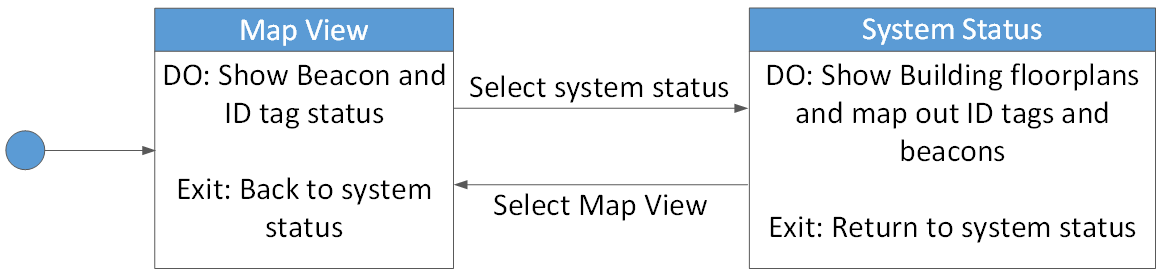
\includegraphics[scale=0.4]{./images/UI_State_FF.png}
    \caption{UI State Diagram - Primary User}
    \label{UISD-1}
\end{figure}
\medskip

The secondary user will be the administrator of the system. For secondary users the interaction is much more complex and require a more in depth level of user interaction. The secondary user interaction state diagram is shown below.

\medskip
\begin{figure}[H]
\centering
    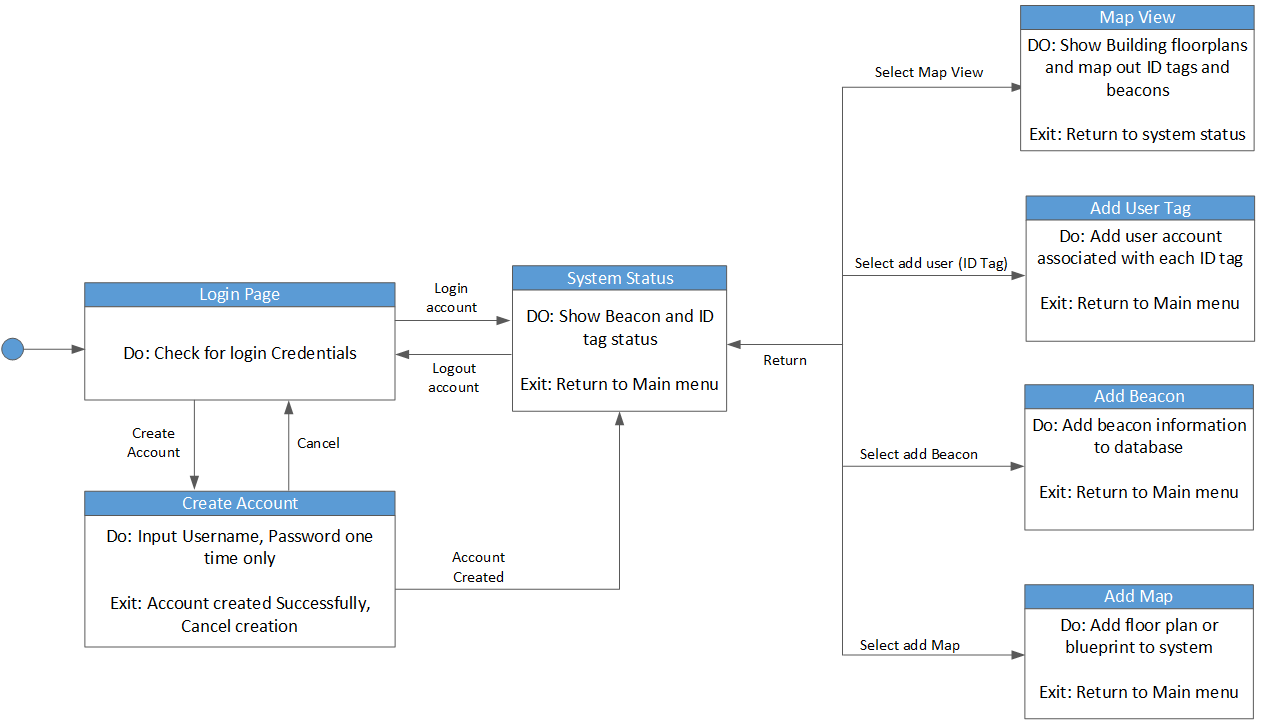
\includegraphics[scale=0.5]{./images/UI_State_IT.png}
    \caption{UI State Diagram - Secondary User}
    \label{UISD-2}
\end{figure}
\medskip



\pagebreak
\subsubsection{UI Mock-Ups}
\medskip
In the Proof of concept a simple console output displaying only the basic information such as the MAC address, RSSI and distance calculations between each beacon and id tag would be shown. Similar to the figure presented below. This UI is just to demonstrate the feasibility of the initial beacon systems.

\medskip
\begin{figure}[H]
\centering
    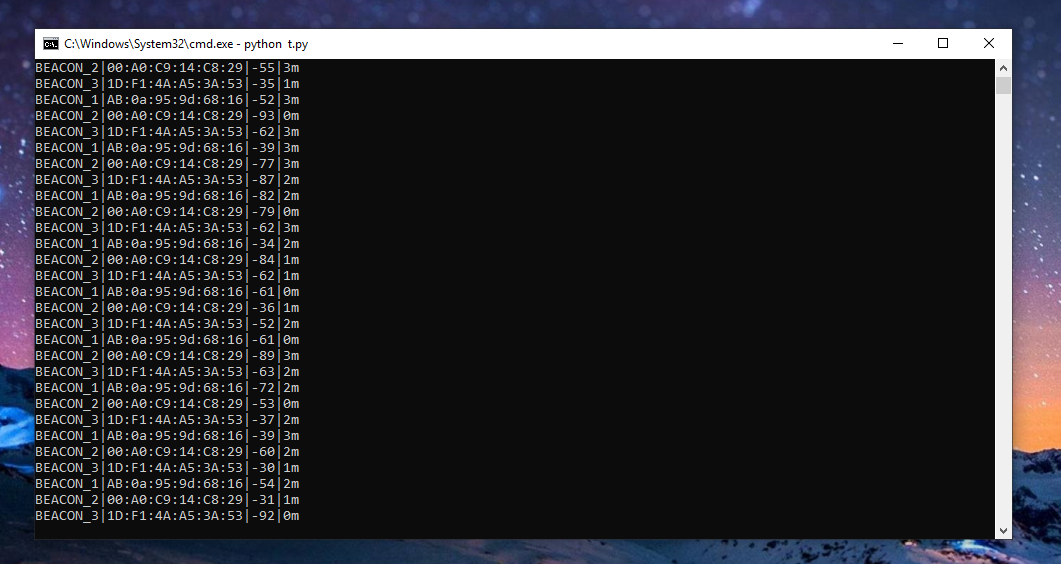
\includegraphics[scale=0.5]{./images/UI_PoC.png}
    \caption{PoC Console UI}
    \label{UI_PoC}
\end{figure}
\medskip

In the prototype phase of development, the user interface would resemble a wireframe of the final implementation. A simple box map is used to display user location in near real time similar to the figure below.

\medskip
\begin{figure}[H]
\centering
    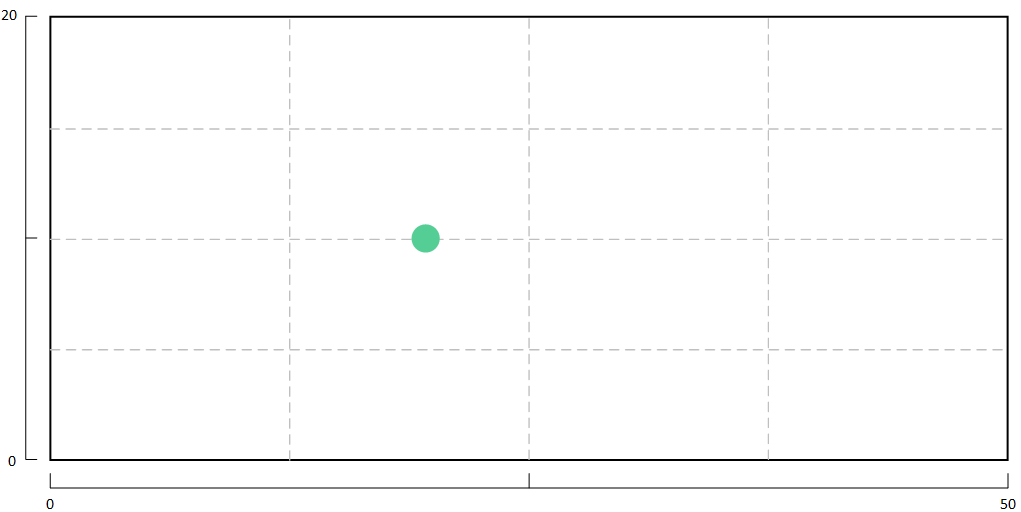
\includegraphics[scale=0.6]{./images/UI_box.png}
    \caption{Prototype Box Map Layout View}
    \label{UI_box}
\end{figure}

\pagebreak

In the Final phase of development the user interface would be complete, resulting in a UI that would fulfil the necessary needs of all users of the system. The primary user would have access to the map view and the system status view shown in figure \ref{map_ff} and \ref{ss_ff}.

\medskip
\begin{figure}[H]
\centering
    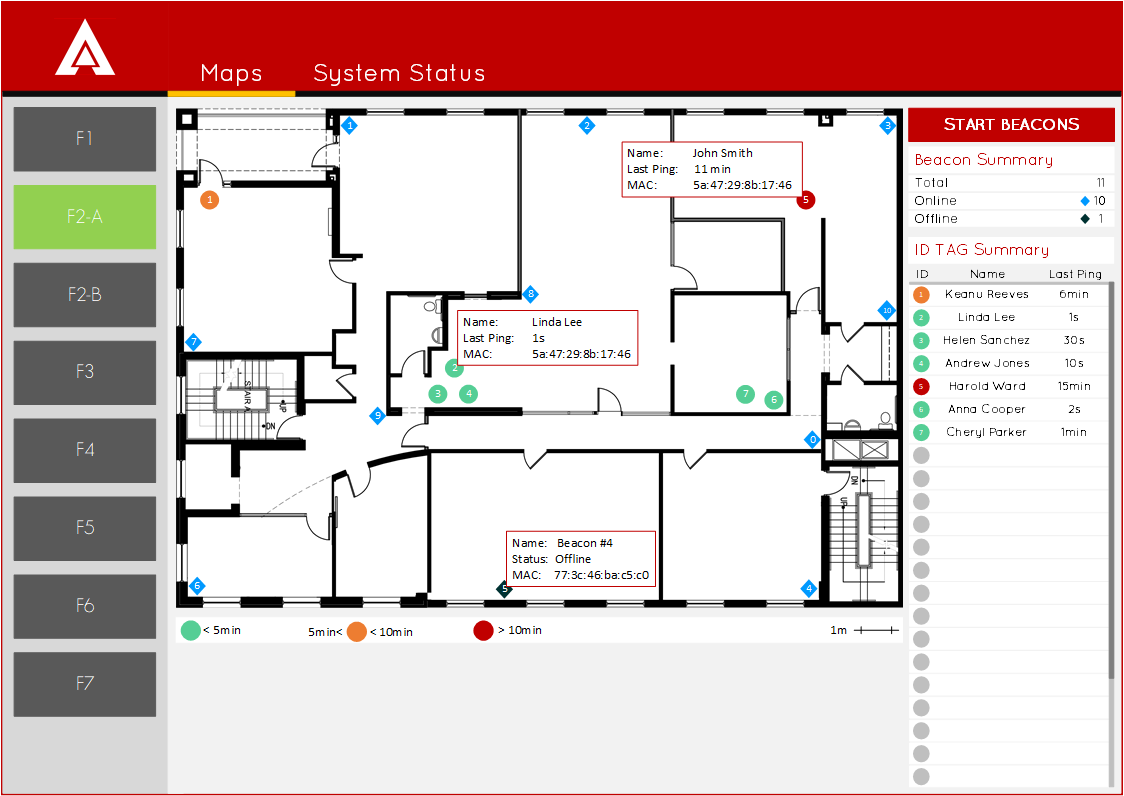
\includegraphics[scale=0.45]{./images/UIMU_map_ff.png}
    \caption{Primary User Map View}
    \label{map_ff}
\end{figure}

\begin{figure}[H]
\centering
    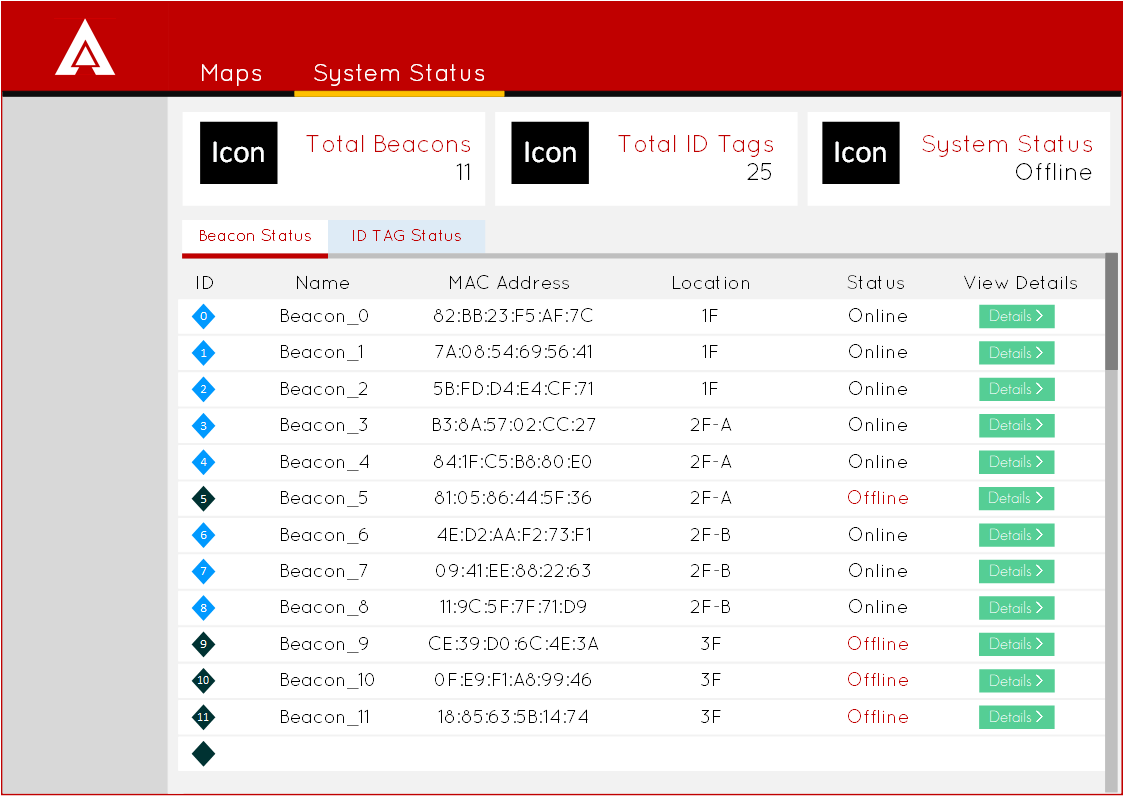
\includegraphics[scale=0.45]{./images/UIMU_status_ff.png}
    \caption{Primary User system status View}
    \label{ss_ff}
\end{figure}
\medskip

\pagebreak
The secondary user, the system administrator will be interacting with the system configurations. The administrator will be performing tasks such as adding/edit beacons, users, and maps or floor plans. The GUI for secondary users are shown in the below figures.

\medskip
\begin{figure}[H]
\centering
    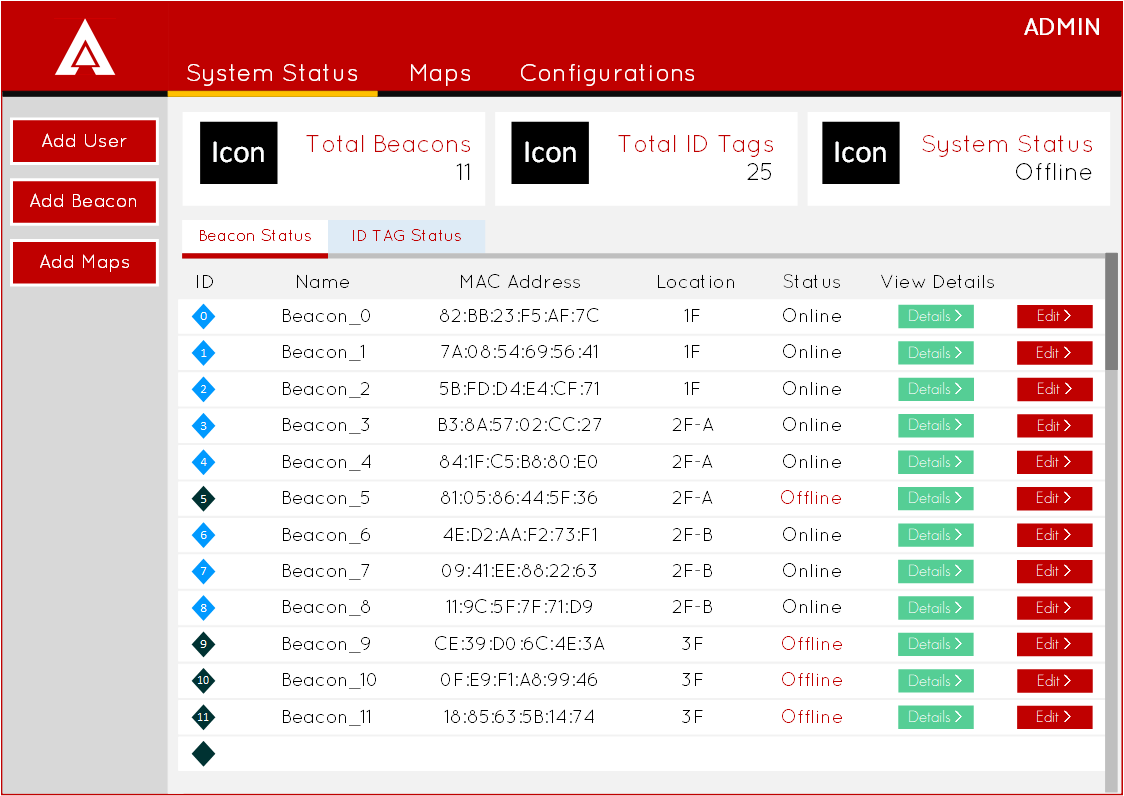
\includegraphics[scale=0.45]{./images/UIMU_status_IT.png}
    \caption{Secondary User System Status View}
    \label{ss_it}
\end{figure}

\medskip
\begin{figure}[H]
\centering
    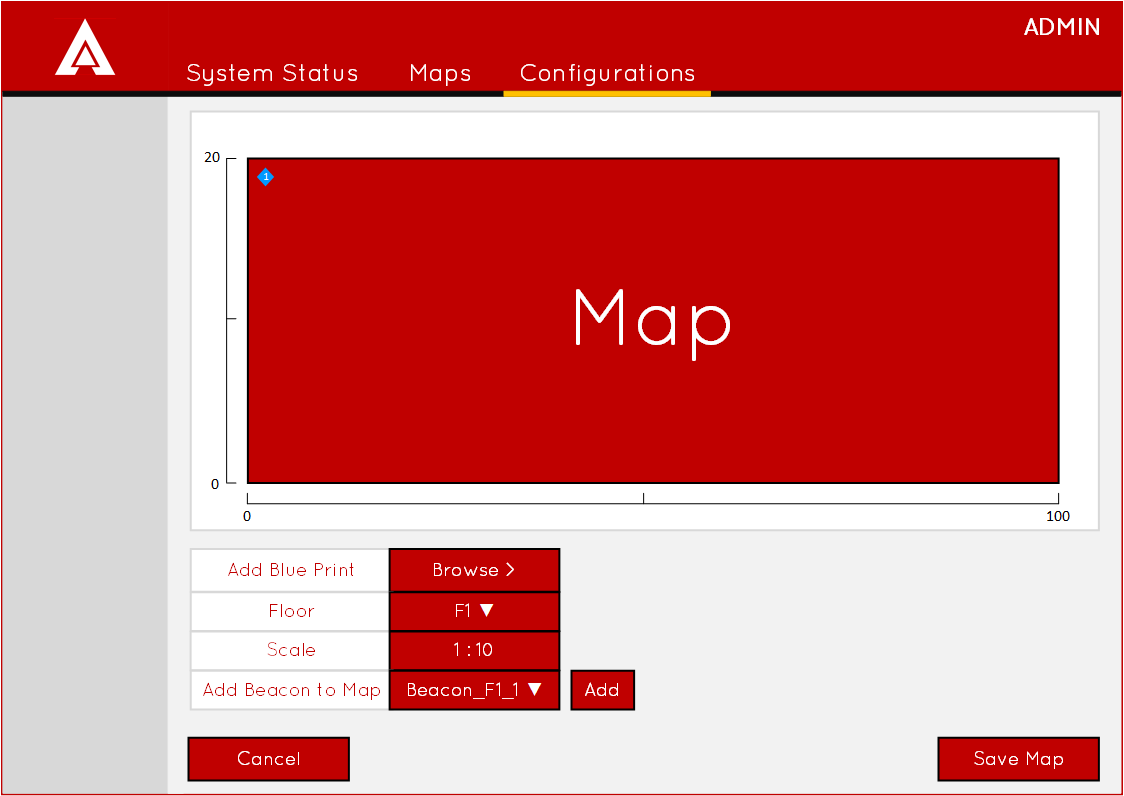
\includegraphics[scale=0.45]{./images/UIMU_add_map.png}
    \caption{Add Map View}
    \label{add_map}
\end{figure}
\pagebreak


\medskip
\begin{figure}[H]
\centering
    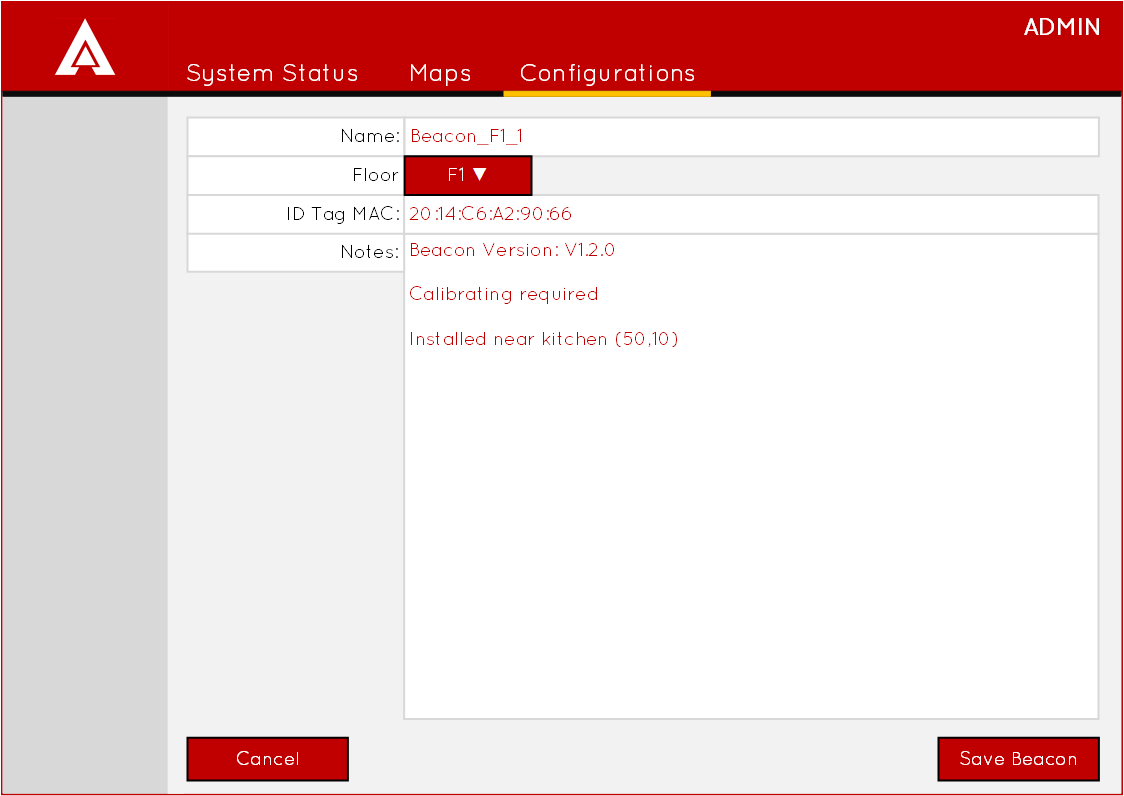
\includegraphics[scale=0.45]{./images/UIMU_add_beacon.png}
    \caption{Add Beacon View}
    \label{add_b}
\end{figure}

\medskip
\begin{figure}[H]
\centering
    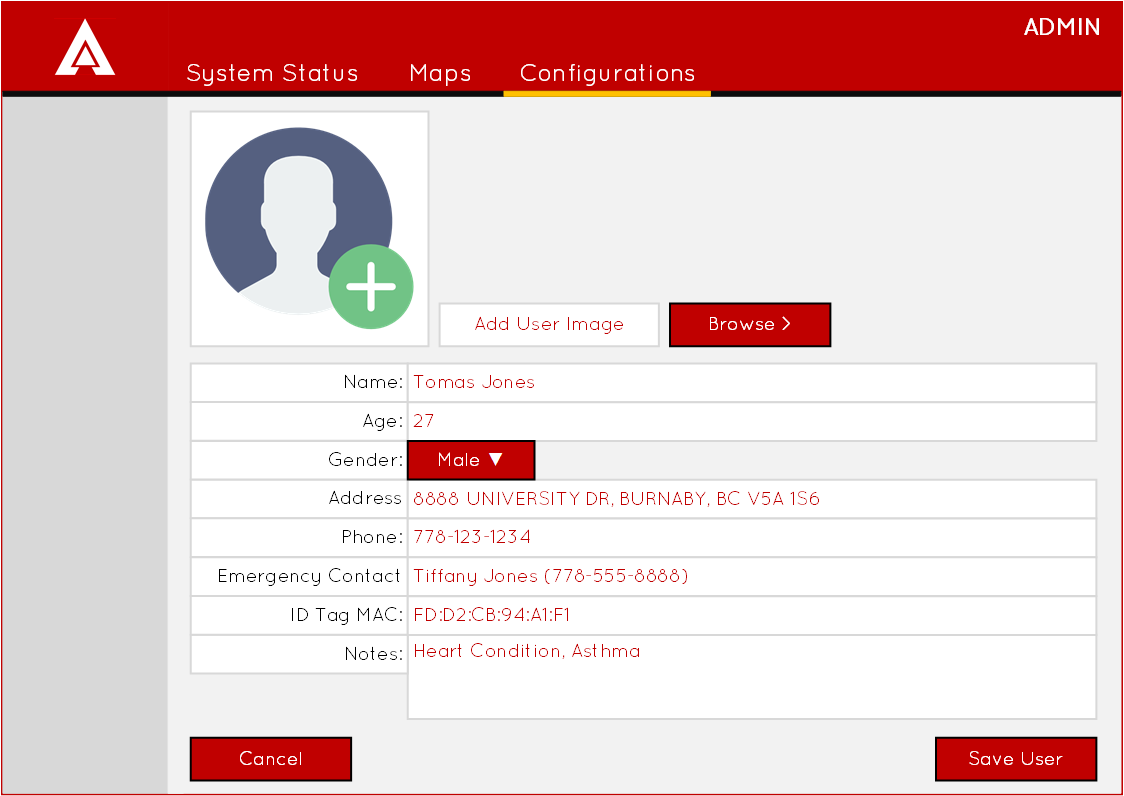
\includegraphics[scale=0.45]{./images/UIMU_add_user.png}
    \caption{Add User View}
    \label{add_user}
\end{figure}






\pagebreak


\subsection{Engineering Standards}
\bigskip
To create an intuitive user interface for optimal user experience, the team at TRIWAVE SYSTEMS will be following several Engineering Standards throughout the development of for the Akriveia Beacon system user interface. The proposed user interface features two branch of components, hardware and software. The hardware components comprising of electronic components such as UWB radio modules and micro-controllers for the device. The software components is split up between data collection from the hardware and data processing. The software also serves as a point of communication and control for the user. The two branches should always inform the user of system operations with easy to understand and highly visible status displayed through the user interface. Interface should also designed in a way that potential errors are kept to a minimum.

\bigskip
These engineering standards published by the \Gls{IEEE}, the \Gls{IEC}, the \Gls{ISO}, and the \Gls{CSA} Group will ensure an intuitive, safe and reliable user interface. Note that some of the standards pertain to the user interface while others pertain to general safety guidelines. The Akriveia Beacon UI design will be built by and tested against the engineering standards listed in the following table.
\bigskip

\def\arraystretch{1.5}
\begin{table}[H]
\centering
\begin{tabular}{ | p{3.5cm} | p{11.5cm}| } 
\hline
\rowcolor{lightgray} \multicolumn{1}{|r|}{\textbf{Standard Code}} & \textbf{Description}\\ 
\hline
\multicolumn{1}{|r|}{CSA-C22.2 NO.61508-1:17} & Functional safety of electrical/electronic/programmableelectronic safety-related systems - Part 1: General requirements \cite{R10-5-1}\\ 
\hline
\multicolumn{1}{|r|}{IEEE 1621-2004} & User Interface Elements in Power Control of Electronic Devices Employed in Office/Consumer Environments \cite{R10-5-2}\\ 
\hline
\multicolumn{1}{|r|}{IEC TR 61997} & Guidelines for the user interface and accompanying word choices \cite{R10-5-3} \\ 
\hline
\multicolumn{1}{|r|}{ISO 20282} & Ease of operation for everyday products \cite{R10-5-4} \\ 
\hline
\multicolumn{1}{|r|}{IEC TR 61997} & Guidelines for the User Interface in Multimedia Equipment for General Purpose Use \cite{R10-5-5} \\ 
\hline
\multicolumn{1}{|r|}{IEEE P360} & Standard for wearable consumer electronic devices \cite{R10-5-6}\\ 
\hline
\multicolumn{1}{|r|}{C22.2 NO.0.23-15} & General Requirements for Battery-Powered Appliances \cite{R10-5-7}\\ 
\hline
\multicolumn{1}{|r|}{IEC 60417} & Graphical symbols for use on equipment \cite{R10-5-8}\\ 
\hline
\multicolumn{1}{|r|}{IEC 62366-1} & Guidance on Usability engineering for software \cite{R10-5-9}\\ 
\hline
\multicolumn{1}{|r|}{ISO/IEC 26907:2009} & Information technology -- Telecommunications and information exchange between systems -- High-rate ultra-wideband PHY and MAC standard \cite{R10-5-10} \\
\hline
\multicolumn{1}{|r|}{ISO/IEC 24730-62:2013} & Information technology -- Real time locating systems (RTLS) -- Part 62: High rate pulse repetition frequency Ultra Wide Band (UWB) air interface \cite{R10-5-11}\\ 
\hline
\end{tabular}
\caption{Engineering Standards}
\end{table}	










\pagebreak


\subsection{Analytical Usability Testing}
\bigskip
The Akriveia beacon user interface will be tested to determine the state of its usability at various stages of development. The analytical testing phase outlines testing procedure that will be done by the engineering and design team using heuristic usability evaluations. Each evaluator will independently examine the UI and check for compliance and usability. After collecting the results the team will discuss and compile possible solutions to usability issues and generate a list of solutions. Finally, the redesign will be implemented and regression testing will be done. The analytical usability testing will take place during the prototype and final product phases of development as the user interface is well defined during these two stages. The testing procedure will follow the steps described below.

\bigskip



\textbf{Step 1:} Usability Research Data Collection\\
\medskip
The first step is to collect the data generated by the usability test. Each evaluator will perform simple tasks outlined in the testing appendix (section \#). From the procedures performed issues will be highlighted and documented. Each issue will have the following:
\begin{itemize}
\setlength\itemsep{0.1mm}
	\item An issue identification (ID).
	\item Note where it happened (screen, module, UI widget, flow, etc.).
	\item Task the user was engaging in.
	\item Concise description of the issue.
\end{itemize}
Data collected will be shown in a table similar to the table below:

\def\arraystretch{1.5}
\begin{table}[H]
\centering
\begin{tabular}{ | p{0.5cm} | p{2cm}| p{5cm} | p{5cm} | p{0.5cm} | p{0.5cm} | p{0.5cm}|} 
\hline 
ID & Where & Task & Description & P1 & P2 & P3 \\
\hline
1 & Login Page & Login with wrong Password & No error message for wrong user name input & X & - & - \\
\hline
2 & Map View & Click on beacon icon & Beacon info text too small & - & X & X \\
\hline
\end{tabular}
\caption{Usability test results}
\end{table}	



\textbf{Step 2:} Issue prioritization\\
\medskip
Once sufficient testing has been performed by evaluators of the team, issues must be prioritized as time and resources are limited for this project. Each usability issue receives a grade of severity, influenced by factors such as:
\begin{itemize}
\setlength\itemsep{0.1mm}
	\item Task criticality: Impact on user if the task is not accomplished.
	\item Issue frequency: How many times an issue has occurred with various participants.
	\item Issue impact: How much has it impacted the user trying to accomplish the task.
\end{itemize}

\bigskip



\textbf{Step 3:} Solution Generation\\
\medskip
With the combined feedback and evaluations, the engineers at TRIWAVE SYSTEMS will re-evaluate possible UI designs for each usability issue that occurred during testing to determine the best and optional solution. A list of recommendations and solutions will be generated with usability test results. For each design decision several alternative solutions must be generated to include other possible ways to address the issue. 








\pagebreak


\subsection{Empirical Usability Testing}
\medskip
This section details the completed empirical usability testing with users and outlines the methods of testing required for future implementations. Empirical usability testing will be carried out by the engineers at TRIWAVE SYSTEMS to systematically determine the usability of the user interface design of the Akriveia Beacon System. 

\bigskip
During empirical usability testing, testing will be carried out in cycles with real users consists of volunteer participants. The first cycle occurs near the end of the Prototype phase and the second cycle occurs near the end of the Final Product phase. Testing will be done with two small groups of participants that are unfamiliar with project development environment. First group will be asked to perform usability test cases outlined in Appendix A. An observer will document actions and observations of the testing process as well as to keep note of average time to complete each task, the amount of errors and error rate, number of tasks completed, and perform a sequence analysis. Issues will be represented similar to the method mentions in 10.6 Analytical usability testing. With the collected data the designers will re-evaluate the user interface for possible solutions for issues. After re-design and implementation a second small group of participants will be asked to perform the same tasks as the first group

\bigskip
From the results generated by participants the following usability elements will be addressed throughout the two testing cycles and development stages. 

\medskip
\begin{itemize}
\setlength\itemsep{0.1mm}
	\item \textbf{Easability:} The familiarity and intuitiveness of the system and how comfortable the users are with the user interfaces in general. 
	\item \textbf{Navigation:} The reliability of the navigation sequences are, how easy is it for the users to understand paths, and/or short cuts. Can the users easily retrace their steps or go back to previous states if they have made a mistake?
	\item \textbf{Responsiveness:} Does the users receive sufficient feedback from interacting with the system? 
	\item \textbf{Intuitiveness:} How quickly can a new user familiarize themselves with the user interface? Whether or not the users are able to perform tasks within a certain amount of time?
	\item \textbf{Robustness:} Safety and reliability of the device and system are addressed by eliminating or minimizing potential error (slips and mistakes) and enabling error recovery.
\end{itemize}

\medskip
By following these usability testing methods mentioned above for the Akriveia Beacon, the engineers and designers at TRIWAVES SYSTEMS can ensure a reliable and intuitive user interface will be produced to meet the needs of its end users. 

\pagebreak


\subsection{Conclusion}
\medskip
The User Interface design for the proof-of-concept, prototype, and the final product of the Akrieva Beacon system developed by TRIWAVE SYSTEMS is detailed in this appendix section. Currently the conceptual framework of the Akriveia Beacon system is under development, with the primary circuitry and initial interfaces under design and early implementations. The major feature to be implemented is the wireless communication interfaces and protocols between anchor beacons and ID tags; the control and data processing unit are also in parallel development. The final project goal is to showcase the Akriveia as an accurate, reliable, modular, and simple solution in providing automated indoor location tracking with near real time and multi-tracking capabilities.  

\bigskip
This appendix outlines a study of the user analysis, and technical analysis for interaction between the system and its intended users. As well as an overview of engineering safety and standards to ensure that the Akriveia Beacon system is safe and reliable for its designated users. Analytical usability testing and empirical usability testing will be performed to ensure that the basic system functionality, aesthetics, stability, and reliability are completely sufficient with of all planned requirements satisfied. 

\bigskip
With the help of the Akriveia Beacon system, under the intended scenario, primary users of the system such as fire fighters and first responders will be able to locate trapped personnel with minimized search time; therefore, lowering rescue time and allowing for higher survival rate for trapped victims during the event of disasters. 














\pagebreak
\printbibliography[title={Appendix References},type=book]
\pagebreak


\end{document}
